% !TEX TS-program = pdflatex
% !TEX encoding = UTF-8 Unicode

% Example of the Memoir class, an alternative to the default LaTeX classes such as article and book, with many added features built into the class itself.

%\documentclass[12pt,a4paper]{memoir} % for a long document
\documentclass[12pt,a4paper,article]{memoir} % for a short document

\usepackage[utf8]{inputenc} % set input encoding to utf8
\usepackage[OT1]{fontenc}
\usepackage[french]{babel}
\usepackage{geometry}

%Pour les marges de la page%
\geometry{left=0.5cm, right=0.5cm, top=0.5cm, bottom=0.5cm}
%Pour les listes à puce%
\frenchbsetup{StandardLists=true} % à inclure si on utilise \usepackage[french]{babel}
\usepackage{enumitem}
\usepackage{amssymb}

%Insertion des images%
\usepackage{graphicx}
\graphicspath{ {./images/} }

% Don't forget to read the Memoir manual: memman.pdf

%%% Examples of Memoir customization
%%% enable, disable or adjust these as desired

%%% PAGE DIMENSIONS
% Set up the paper to be as close as possible to both A4 & letter:
\settrimmedsize{11in}{210mm}{*} % letter = 11in tall; a4 = 210mm wide
\setlength{\trimtop}{0pt}
\setlength{\trimedge}{\stockwidth}
\addtolength{\trimedge}{-\paperwidth}
\settypeblocksize{*}{\lxvchars}{1.618} % we want to the text block to have golden proportionals
\setulmargins{50pt}{*}{*} % 50pt upper margins
\setlrmargins{*}{*}{1.618} % golden ratio again for left/right margins
\setheaderspaces{*}{*}{1.618}
\checkandfixthelayout 
% This is from memman.pdf

%%% \maketitle CUSTOMISATION
% For more than trivial changes, you may as well do it yourself in a titlepage environment
\pretitle{\begin{center}\sffamily\huge\MakeUppercase}
\posttitle{\par\end{center}\vskip 0.5em}

%%% ToC (table of contents) APPEARANCE
\maxtocdepth{subsection} % include subsections
\renewcommand{\cftchapterpagefont}{}
\renewcommand{\cftchapterfont}{}     % no bold!

%%% HEADERS & FOOTERS
\pagestyle{ruled} % try also: empty , plain , headings , ruled , Ruled , companion

%%% CHAPTERS
\chapterstyle{hangnum} % try also: default , section , hangnum , companion , article, demo

\renewcommand{\chaptitlefont}{\Huge\sffamily\raggedright} % set sans serif chapter title font
\renewcommand{\chapnumfont}{\Huge\sffamily\raggedright} % set sans serif chapter number font

%%% SECTIONS
\hangsecnum % hang the section numbers into the margin to match \chapterstyle{hangnum}
\maxsecnumdepth{subsection} % number subsections

\setsecheadstyle{\Large\sffamily\raggedright} % set sans serif section font
\setsubsecheadstyle{\large\sffamily\raggedright} % set sans serif subsection font

%% END Memoir customization

\title{}
\author{}
\date{} % Delete this line to display the current date

%%% BEGIN DOCUMENT
\begin{document}
	
	   \begin{center}
	 	    \textbf{Institut Supérieur des  Etudes Technologiques de Radès}\\\vfill
		    \huge \textbf{P F E} \normalsize \\\vfill
		    Pour l'Obtention d'un\\
	           \Large \textbf{Mastère 2}\\
		    \LARGE \textbf{En Business Intelligence}\\ \normalsize\vfill
		    Présenté Et Soutenu Par:  \Large Laby Damaro CAMARA \normalsize\\\vfill
	          \rule{0.95\textwidth}{1.5pt}\\ \vspace{\baselineskip}
		    \Large \textbf{Titre} \normalsize \\\vfill
		    Création d’une application d’identification faciale et de reconnaissance automatique de produits\\
		   \rule{0.95\textwidth}{1.5pt}\\ \vspace{0.9\baselineskip}\vfill
		    Encadré Par Madame: \Large Hind OUEDI\normalsize\\
		    Soutenu le dd/mm/aaaa\\\vfill
	          \begin{tabular}{ll}
	                 \hline\hline
				    \emph{Jury} & ???\\
				    \emph{Rapporteurs} & ???\\
			          \emph{Rapporteurs} & ???\\
	                \hline\hline
	          \end{tabular}
	   \end{center}
\maketitle
\tableofcontents* % the asterisk means that the contents itself isn't put into the ToC

     \newpage
	\chapter{Introduction}
		\begin{itemize}[label=$\star$]
			\item Comment introduire des notions d'intelligence artificielle à des moyens de personnalisation dans le domaine du commerce en ligne;
			\item Quelle est l'utilité de la vision par ordinateur dans le domaine du commerce électronique en général et commerce en ligne en particulier;
			\item Comment interviennent la reconnaissance des produits et la detection de leurs caracteristiques.
	             \item Faire des recherches des produits similaires à travers l'image
		\end{itemize}

	\chapter{Contexte Général}
		\begin{figure}[h!]
			\centering
			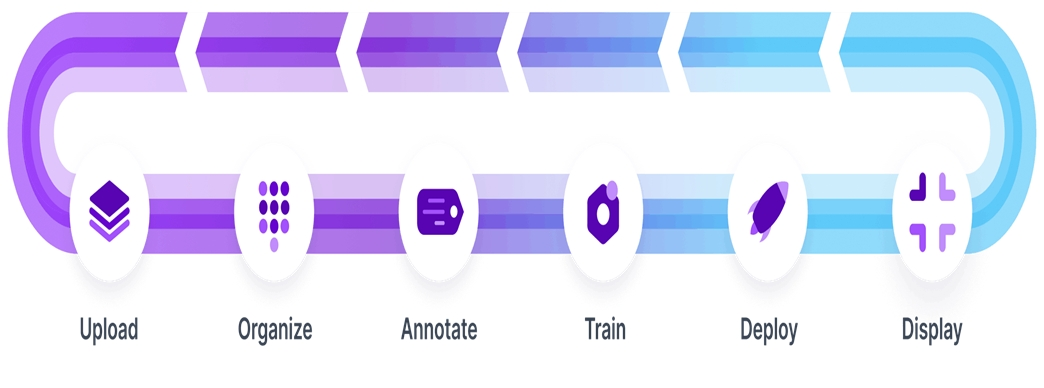
\includegraphics[width=150mm,height=70mm]{visionordinateur}
			\caption{Etape d'un Projet de Vision Par Ordinateur}
			\label{fig:Comment La Vision Par Ordinateur Fonction}
		\end{figure}
	
		\begin{figure}[h!]
			\centering
			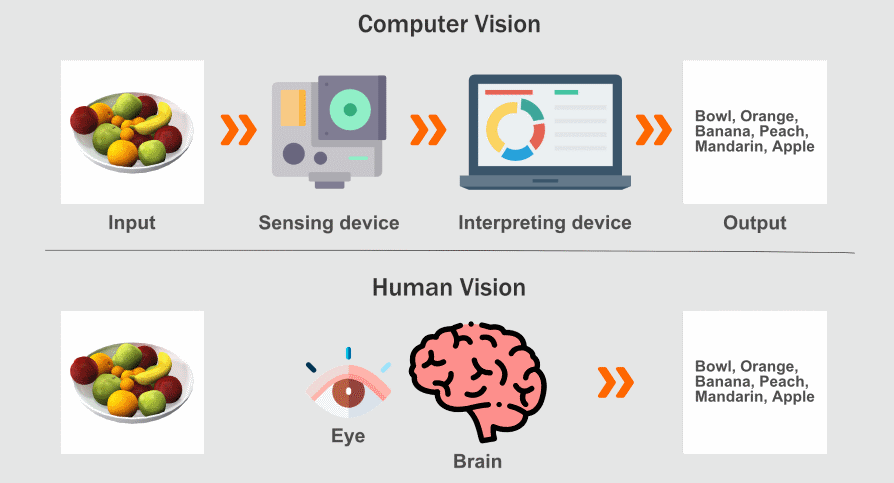
\includegraphics[width=150mm,height=70mm]{howdoesvomputervisionwork}
			\caption{Comment La Vision Par Ordinateur Fonction}
			\label{fig:Comment La Vision Par Ordinateur Fonction}
		\end{figure}
 		\begin{figure}[h!]
			\centering
			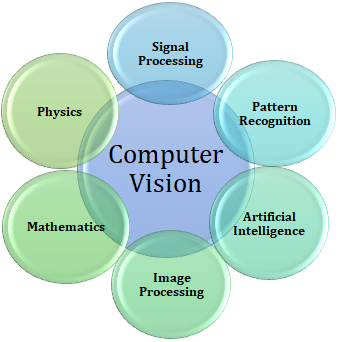
\includegraphics[width=150mm,height=80mm]{mainknowlegecv}
			\caption{Les Compétences Requises Pour ce Projet}
			\label{fig:Les Compétences Requises Pour ce Projet}
		\end{figure}	
			
		\begin{figure}[h!]
			\centering
			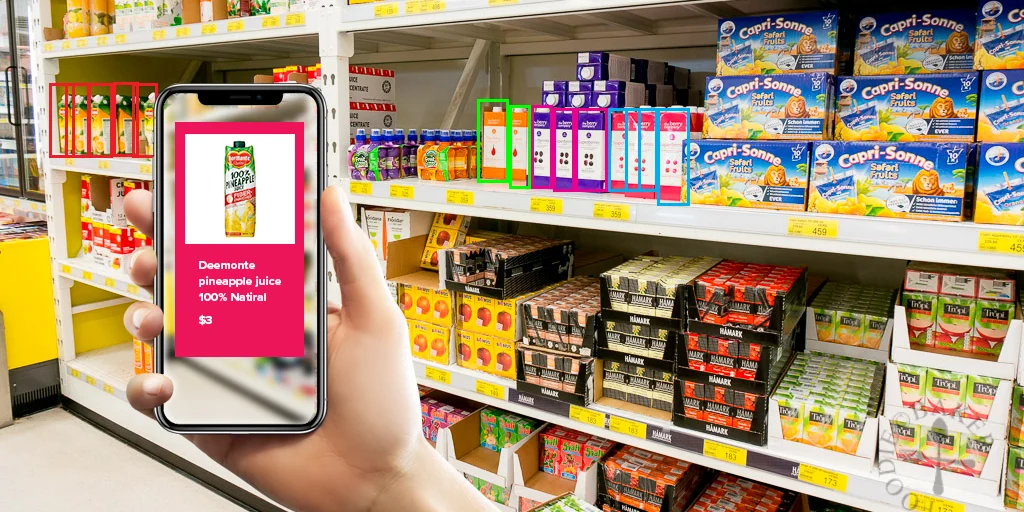
\includegraphics[width=150mm,height=70mm]{productdetect}
			\caption{product detected produit Par Image}
			\label{fig:product detected produit Par Image}
		\end{figure}

 
\end{document}
